\documentclass[10pt]{beamer}

\usetheme{metropolis}
\usepackage{appendixnumberbeamer}

\usepackage{booktabs}
\usepackage[scale=2]{ccicons}

\usepackage{pgfplots}
\usepgfplotslibrary{dateplot}

\usepackage{pgfpages}
%\setbeameroption{show notes} %Notizen anzeigen
%\setbeameroption{show notes on second screen = left}


\usepackage{xspace}
\newcommand{\themename}{\textbf{\textsc{metropolis}}\xspace}

\usepackage{color}

\definecolor{codegreen}{rgb}{0,0.6,0}
\definecolor{codegray}{rgb}{0.5,0.5,0.5}
\definecolor{codepurple}{rgb}{0.58,0,0.82}
\definecolor{backcolour}{rgb}{0.95,0.95,0.92}
\definecolor{airforceblue}{rgb}{0.36, 0.54, 0.66}
\definecolor{maroon}{rgb}{0.5, 0.0, 0.0}

\usepackage{listings}
\lstdefinestyle{mystyle}{
	backgroundcolor=\color{backcolour},   
	commentstyle=\color{codegreen},
	keywordstyle=\color{magenta},
	numberstyle=\tiny\color{codegray},
	stringstyle=\color{codepurple},
	basicstyle=\fontsize{8}{10}\selectfont\ttfamily,
	breakatwhitespace=false,         
	breaklines=true,                 
	captionpos=b,                    
	keepspaces=true,                 
	numbers=left,                    
	numbersep=5pt,                  
	showspaces=false,                
	showstringspaces=false,
	showtabs=false,                  
	tabsize=2
}
\lstset{style=mystyle}

\usepackage{diagbox}

\usepackage{tikz}
\usetikzlibrary{fit,shapes.geometric}

\newcounter{nodemarkers}
\newcommand\circletext[1]{%
	\tikz[overlay,remember picture] 
	\node (marker-\arabic{nodemarkers}-a) at (0,1.5ex) {};%
	#1%
	\tikz[overlay,remember picture]
	\node (marker-\arabic{nodemarkers}-b) at (0,0){};%
	\tikz[overlay,remember picture,inner sep=2pt]
	\node[draw,ellipse,fit=(marker-\arabic{nodemarkers}-a.center) (marker-\arabic{nodemarkers}-b.center)] {};%
	\stepcounter{nodemarkers}%
}



\title{Rucksack Problem}
\subtitle{Algorithmen und Datenstrukturen II}
\date{\today}
\author{Sebastian Baumann, Korbinian Karl, Ehsan Moslehi}
\institute{Hochschule für Angewandte Wissenschaften München}
%\titlegraphic{\hfill\includegraphics[height=1.5cm]{logo.pdf}}

\begin{document}

\maketitle

\begin{frame}{Table of contents}
  \setbeamertemplate{section in toc}[sections numbered]
  \tableofcontents[hideallsubsections]
\end{frame}

\section{Beschreibung des Problems}

\begin{frame}[fragile]{Rucksack Problem}
	\begin{figure}
		\centering
		
\includegraphics[width=1\linewidth]{images/rp}
		\caption{Rucksack Problem}
		\label{fig:rp}
	\end{figure}
\end{frame}

\begin{frame}[fragile]{Mathematische Beschreibung}
	\textbf{Gegeben:}
	\begin{itemize}
		\item Ggegenstände $1, 2, 3 , ..., n$
			\begin{itemize}
				\item $w_{i}$ : Wert vom Gegenstand $i$
				\item $v_{i} \in \mathbb{N}$ : Volumen vom Gegenstand $i$
			\end{itemize}
		\item Rucksack mit dem Volumen $V \in \mathbb{N}$
	\end{itemize}
	
	\textbf{Gesucht:}\\ 
	\vspace{0.3cm}
	\hspace{0.3cm}
	Eine Rucksackfüllung mit maximalen Gesamtwert, wobei das Volumen $V$ nicht überschritten werden darf.\\
	\vspace{0.3cm}
	\begin{center}
		$max \Big\lbrace \sum \limits_{i=1}^{n} w_{i}t_{i} \mid \sum \limits_{i=1}^{n} v_{i}t_{i} \leq V , \forall i : t_{i} \in \{0, 1\} \Big\rbrace$
	\end{center}
\end{frame}

\begin{frame}[fragile]{Mathematische Beschreibung}
	\begin{itemize}[<+- | alert@+>]
		\item[] \begin{center}
			Ganzzahliges Lineares Optimierungsproblem
		\end{center}
		\item[] \begin{center}
			\textbf{NP-Vollständig}
		\end{center}
	\end{itemize}
\end{frame}

\section{Lösungsansätze}

\begin{frame}[fragile]{Brute Force}
	\begin{enumerate}
		\item Brute Force
		\item Greedy
		\item Dynamische Programmierung 
	\end{enumerate}
\end{frame}

\section*{Brute Force}

\begin{frame}[fragile]{Brute Force}
	\begin{figure}
		\centering
		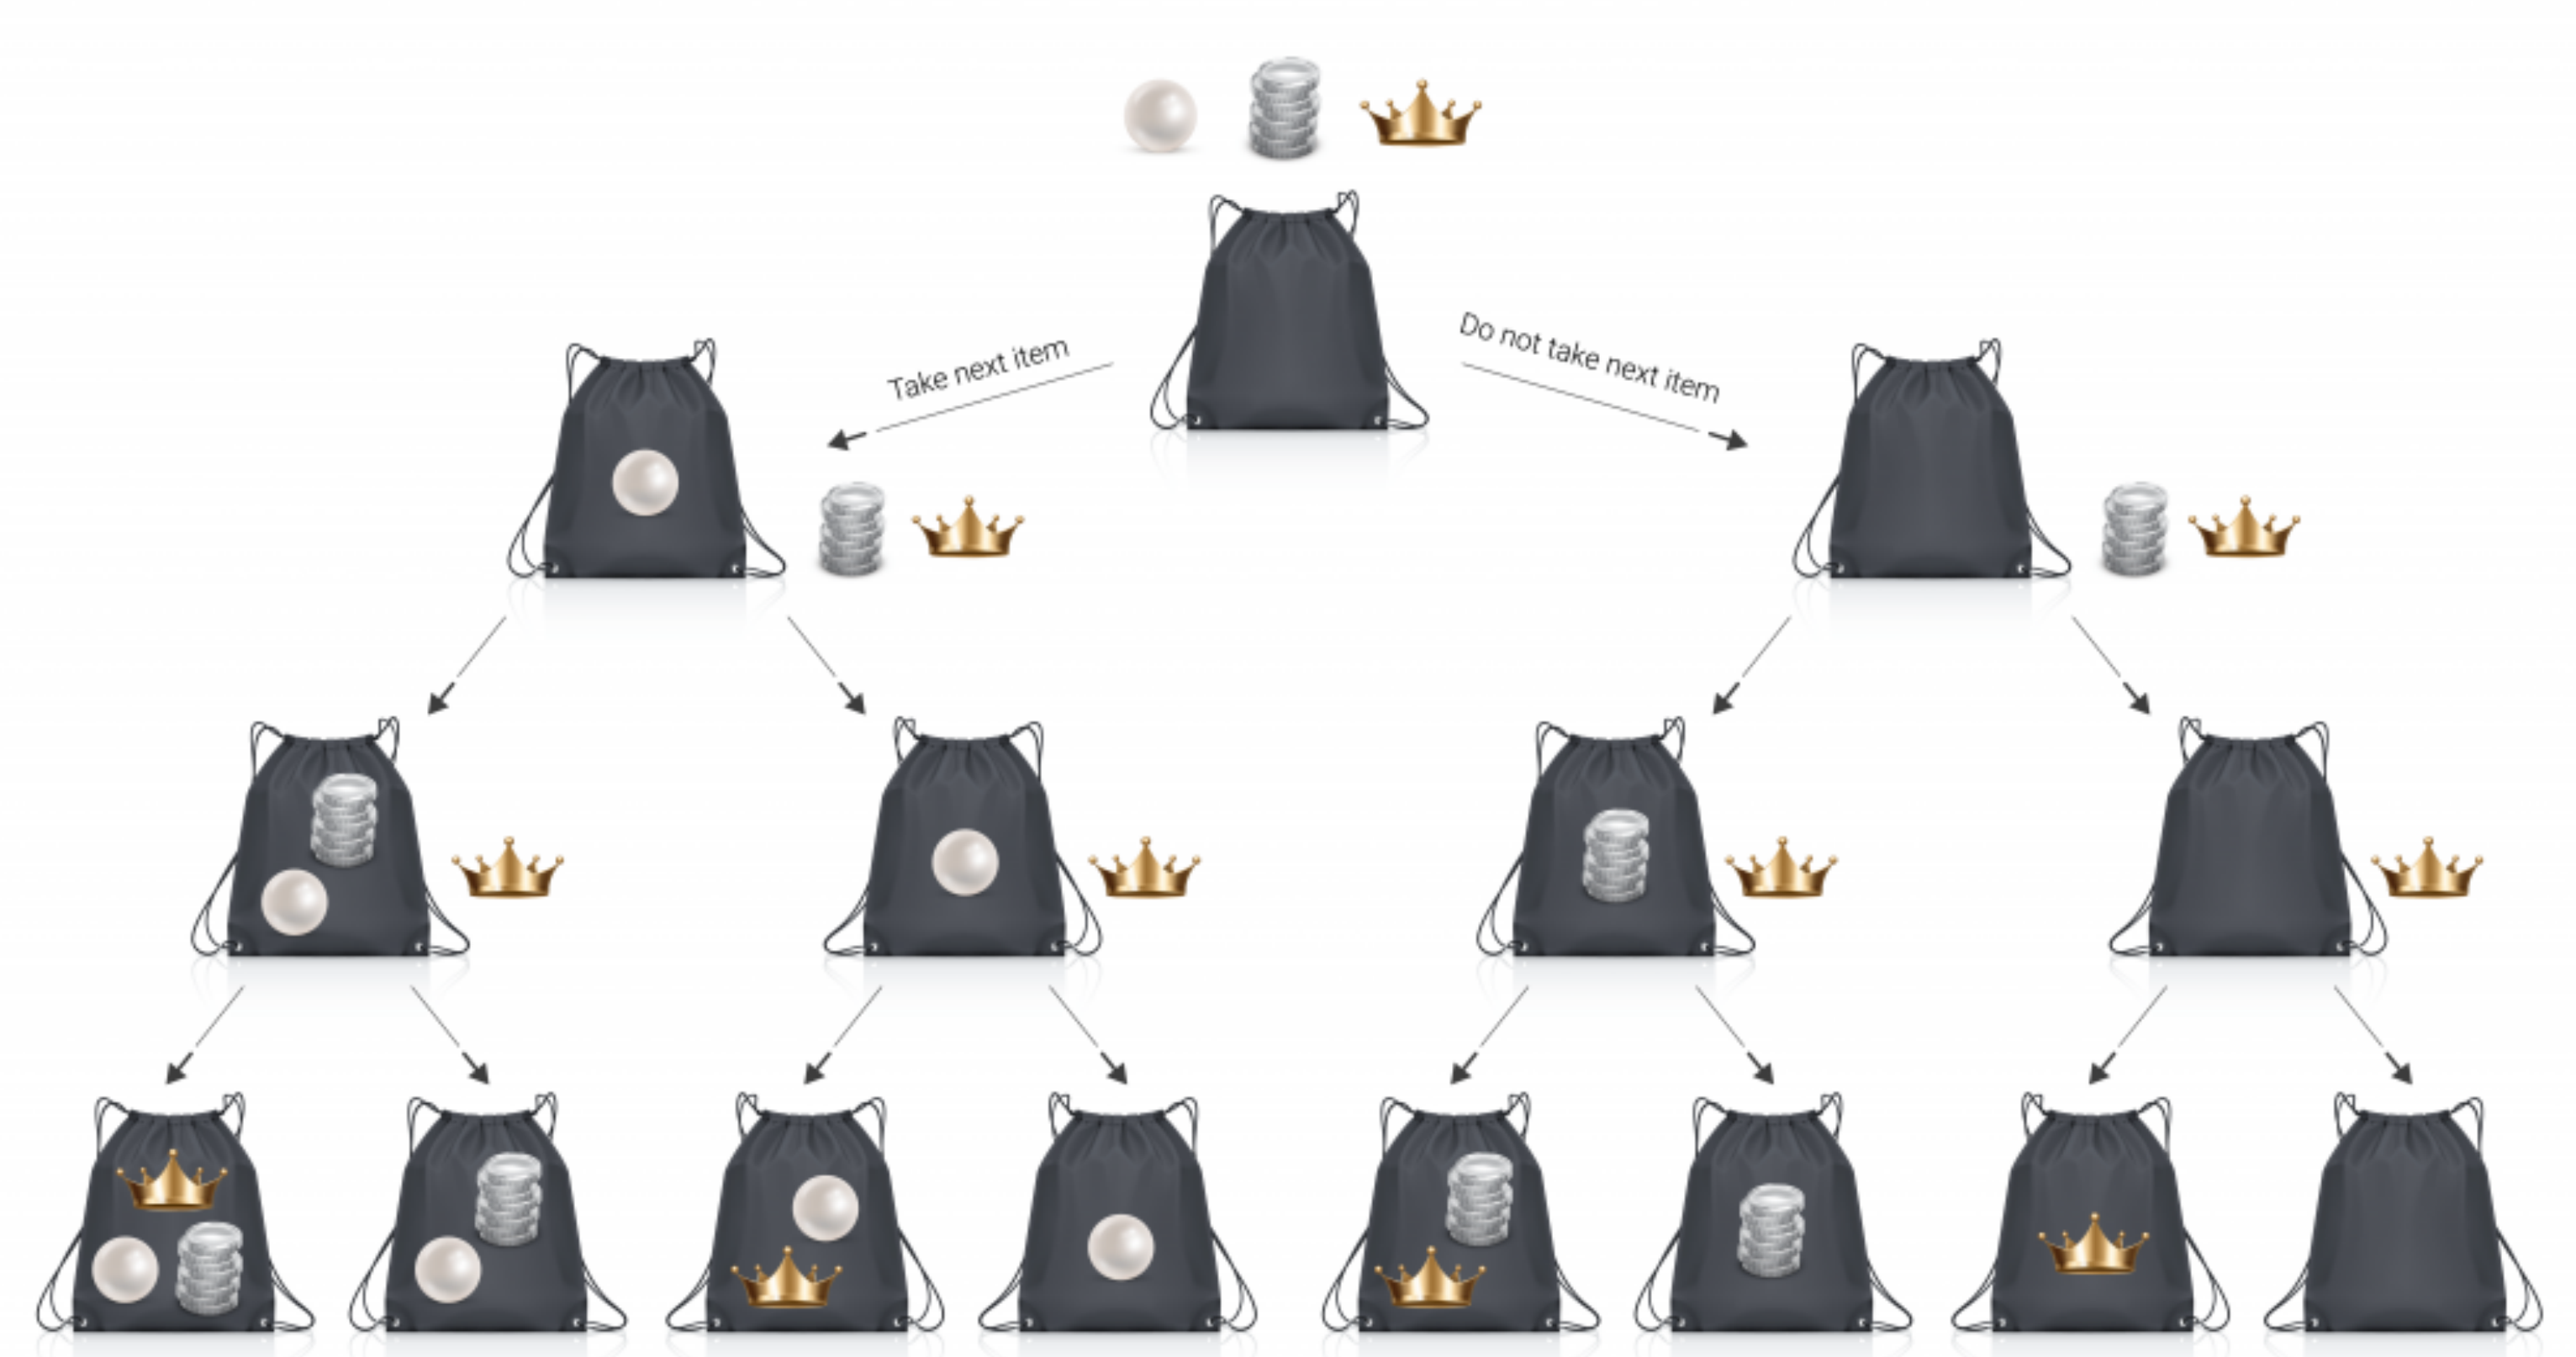
\includegraphics[width=1\linewidth]{images/rp-bf}
		\caption{Probiere alle Teilmengen!}
		\label{fig:rp-bf}
	\end{figure}
\end{frame}

\begin{frame}[fragile]{Brute Force}
	\begin{itemize}[<+- | alert@+>]
		\item[] \begin{center}
			\textbf{Optimale globale Lösung wird gefunden.}
		\end{center}
	\vspace{1cm}
		\item[] \begin{center}
			\textbf{Exponentielle Laufzeit $O(2^n)$}
		\end{center}
	\end{itemize}
\end{frame}

\section*{Greedy Algorithmus}

\begin{frame}[fragile]{Greedy Strategie}
	\textbf{Strategien:}
	\begin{enumerate}[<+- | alert@+>]
		\item \textbf{Absteigende Sortierung nach Wert}
		\item \textbf{Aufsteigende Sortierung nach Volumen}
		\item \textbf{Absteigende Sortierung nach Wertdichte} \Large{ $d_{i} = \frac{w_{i}}{v_{i}}$}
	\end{enumerate}
	\vspace{1cm}
	\textbf{Packe solange Gegenstände in den Rucksack, bis kein Gegenstand mehr rein passt!}
\end{frame}

\begin{frame}[fragile]{Greedy Strategie}
	\begin{itemize}[<+- | alert@+>]
		\item[] \begin{center}
			\textbf{Optimale globale Lösung wird \Large{NICHT} \normalsize{gefunden}.}\\
			\textbf{Optimale lokale Lösung wird gefunden.}
		\end{center}
		\vspace{1cm}
		\item[] \begin{center}
			\textbf{Laufzeit $O(n. \log n)$}
		\end{center}
	\end{itemize}
\end{frame}

\section*{Dynamische Programmierung}

\begin{frame}[fragile]{Dynamische Programmierung}
	\begin{enumerate}[<+- | alert@+>]
		\item Teile das Problem in gleichartige Teilprobleme!
		\item Speichere die Resultate der Teilprobleme systematisch, um wiederholte Berechnungen zu vermeiden!
		\item Setze die optimale Lösung aus den optimalen Lösungen der Teilprobleme zusammen!
	\end{enumerate}
\end{frame}

\begin{frame}[fragile]{Dynamische Programmierung}
	\textbf{Idee:}
	\begin{enumerate}[<+- | alert@+>]
		\item Löse das Problem für eine Menge von Gegenständen mit einem Gegenstand und einem Rücksack mit Volumen eins. Speichere das Ergebnis in einer Tabelle.
		\item Wiederhole das für verschiedene Rucksäcke mit volumen $2, ..., V$ und benutze dabei die vorherige Ergebnisse.
		\item Wiederhole die vorherigen Schritte für Mengen mit zwei, drei, ..., n Gegenständen.		
	\end{enumerate}
\end{frame}

\begin{frame}[fragile]{Dynamische Programmierung}
		\begin{lstlisting}[language=go]
		for i := 1; i <= numItems; i++ {
			for j := 1; j <= capacity; j++ {
				if is[i-1].volume <= j {
					valueOne := float64(matrix[i-1][j])
					valueTwo := float64(is[i-1].worth + matrix[i-1][j-is[i-1].volume])
					matrix[i][j] = int(math.Max(valueOne, valueTwo))
				} else {
					matrix[i][j] = matrix[i-1][j]
				}
			}
		}			
		\end{lstlisting}
\end{frame}
	
\begin{frame}[fragile]{Dynamische Programmierung}
	\textbf{Beispiel:}
	\begin{itemize}
		\item[] Rucksack mit Volumen 5.
		\item[] Gegenstände :
		\begin{enumerate}
			\item $v_{1} = 3, w_{1} = 5$
			\item $v_{2} = 2, w_{2} = 3$
			\item $v_{3} = 1, w_{3} = 4$
		\end{enumerate} 
	\end{itemize}
\end{frame}
		
\begin{frame}[fragile]{Dynamische Programmierung}
	\begin{center}
		\textbf{Fülle die Tabelle!}
	\end{center}
	\begin{center}
		\begin{tabular}{|l||p{0.5cm}|p{0.5cm}|p{0.5cm}|p{0.5cm}|p{0.5cm}|}
		\hline
		\diagbox{I:}{V:}
		& 1 & 2 & 3 & 4 & 5 \\
		\hline
		1 (3, 5)	&    0    &     0     &      5      &       5      &       5     \\
		\hline
		2 (2, 3)	&    0    &     3     &      5      &       5      &       8     \\
		\hline
		3 (1, 4)	&    4    &     4     &      7      &       9      &       9     \\
		\hline
	\end{tabular}

	\end{center}

\end{frame}

\begin{frame}[fragile]{Dynamische Programmierung}
	\begin{itemize}
		\item Fange unten Rechts an.
		\item Vergleiche den Wert mit dem Wert in der Zelle drüber.
			\begin{enumerate}
				\item Die Werte sind gleich $\Rightarrow$ Der Gegenstand ist nicht genommen.
				\item Die Werte sind nicht gleich $\Rightarrow$ Der Gegenstand genommen. So gehe eine Zeile hoch und um Volumen vom Gegenstand nach links. 
			\end{enumerate}
		\item Wiederhole bis der Zeiger aus der Tabelle raus geht.
	\end{itemize}
	\begin{center}
		\begin{tabular}{|l||p{0.5cm}|p{0.5cm}|p{0.5cm}|p{0.5cm}|p{0.5cm}|}
			\hline
			\diagbox{I:}{V:}
			& 1 & 2 & 3 & 4 & 5 \\
			\hline
			1 (3, 5)	&    0    &     0     &      5      & \circletext{5}      &       5     \\
			\hline
			2 (2, 3)	&    0    &     3     &      5      & 		5      &       8     \\
			\hline
			3 (1, 4)	&    4    &     4     &      7      &       9      & \circletext{9} \\
			\hline
		\end{tabular}
		
	\end{center}
	
\end{frame}


\begin{frame}[standout]
  Fragen?
\end{frame}

\appendix

%\begin{frame}[allowframebreaks]{References}
%  \bibliography{demo}
%  \bibliographystyle{abbrv}
%\end{frame}

\end{document}
